% Owner: D
% M3a - Temporal Reachability

\begin{figure}[t]
    \centering
    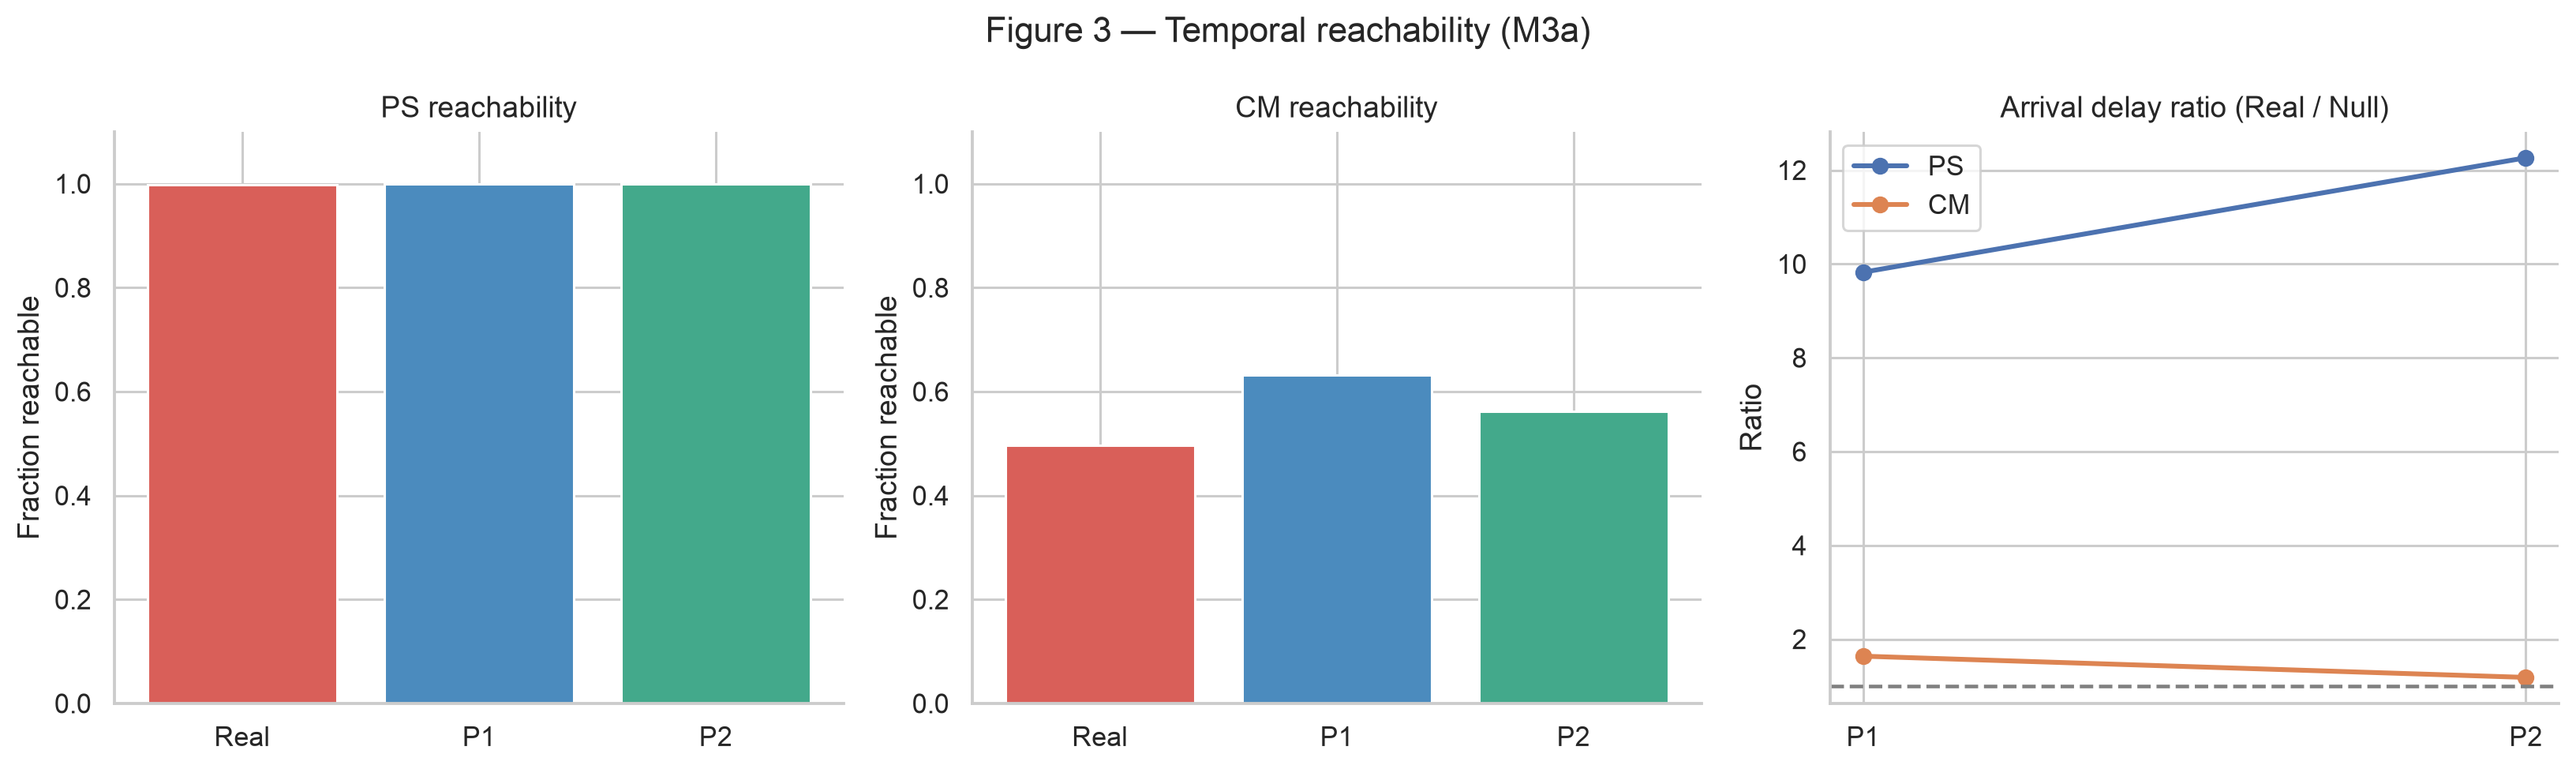
\includegraphics[width=\linewidth]
    {Fig3_reachability_and_delay.png}
    \caption{Temporal reachability comparison
    between real and randomized networks.}
    \label{fig:d_reachability}
\end{figure}

% 后面继续放你的完整M3a实验分析
% =========================================================
% Member D: M3a Temporal Reachability and M3c SIR Spreading
% =========================================================

\subsubsection{Temporal Reachability (M3a)}
\label{sec:d_reachability}

We first investigate H6a: temporal ordering restricts
network reachability. We compare the original temporal
networks (Real) with timestamp-shuffled (P1) and
edge-randomized (P2) reference networks.

Two metrics are considered: temporal reachability and
mean earliest-arrival delay. The former measures the
fraction of reachable nodes under time-respecting paths,
while the latter measures the time required to reach
accessible destinations.

\paragraph{Reachability results.}

Figure~\ref{fig:d_reachability} presents the temporal
reachability results for the Primary School (PS) and
CollegeMsg (CM) datasets.

\begin{figure*}[t]
    \centering
    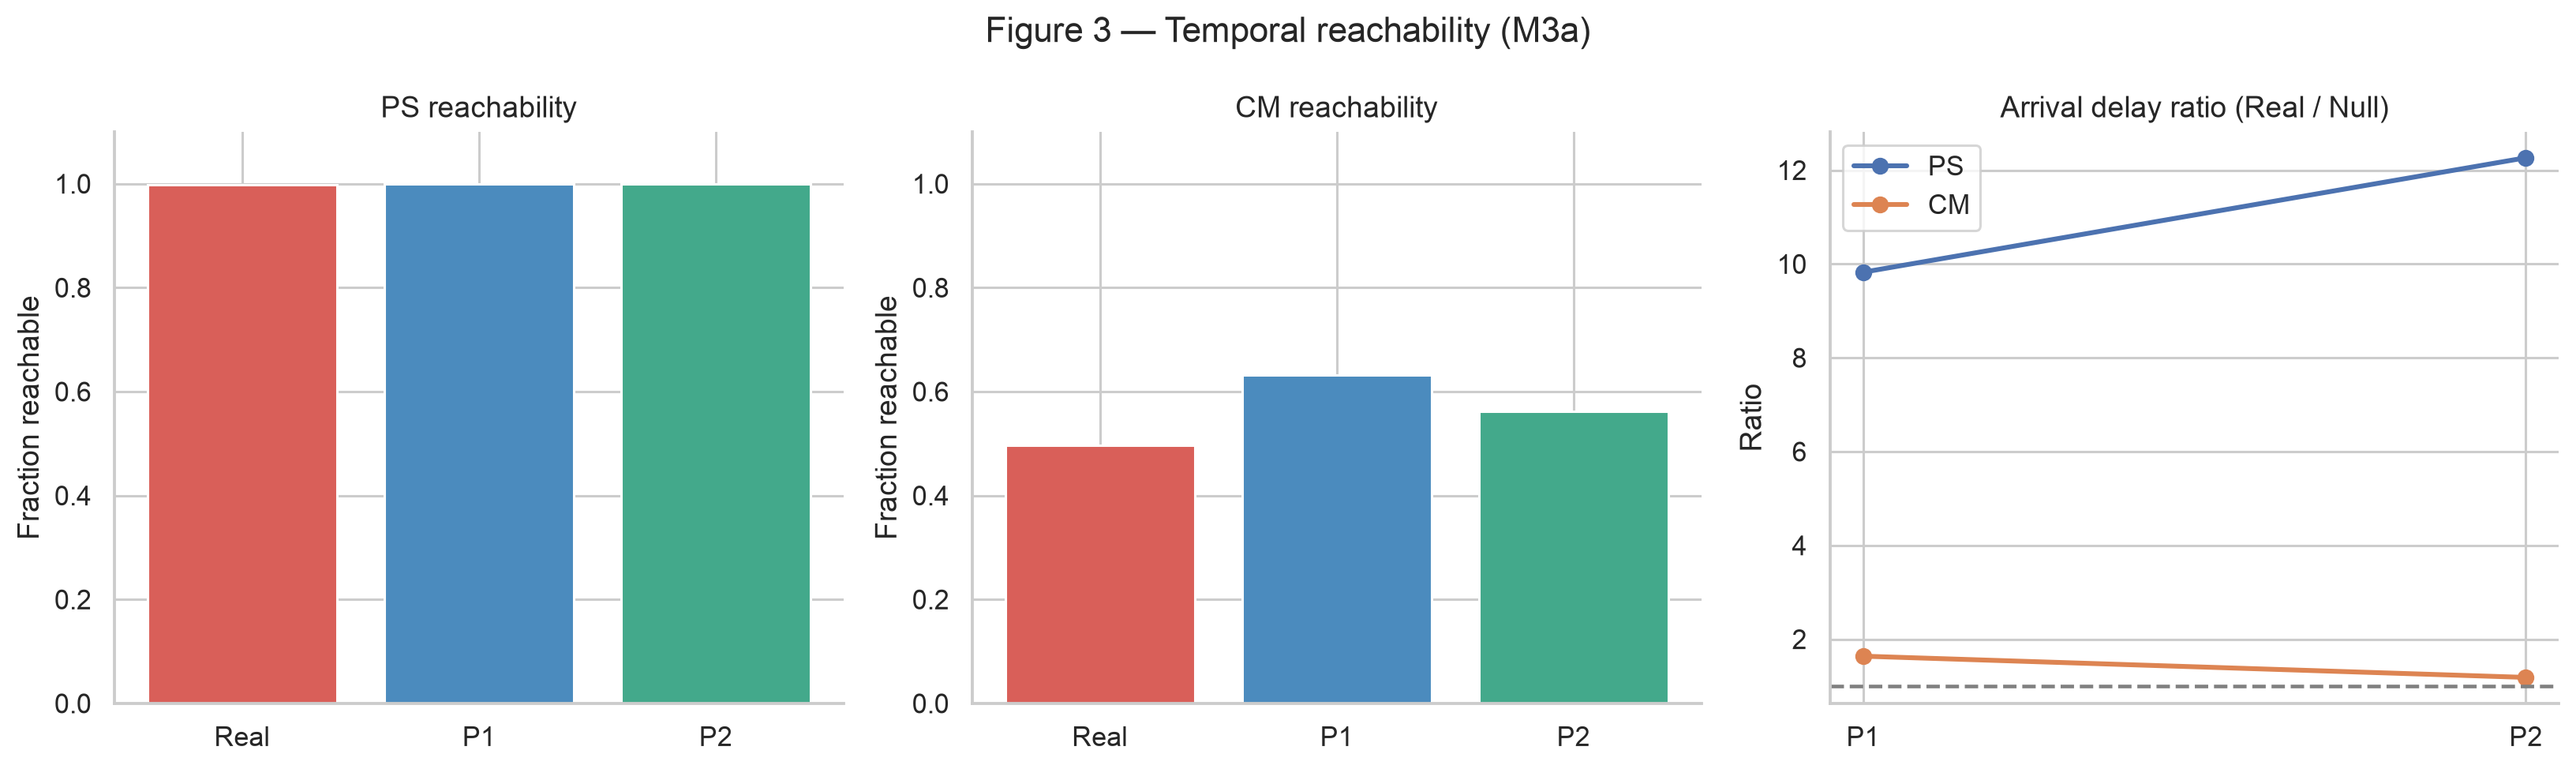
\includegraphics[width=0.85\textwidth]
    {Fig3_reachability_and_delay.png}
    \caption{Temporal reachability analysis (M3a).
    The first two panels show reachability in PS and CM.
    The third panel compares the real-to-null arrival-delay
    ratios. Ratios above one indicate longer arrival delays
    in the original temporal network.}
    \label{fig:d_reachability}
\end{figure*}

In PS, the real network achieves a reachability ratio
of 0.9981, compared with 1.0000 for both P1 and P2.
Thus, almost all nodes remain temporally reachable
regardless of randomization.

However, the mean arrival delay differs substantially.
The real-network delay is approximately 9.82 times
that of P1 and 12.26 times that of P2.

This indicates that temporal ordering does not
necessarily prevent nodes from being reached,
but can considerably delay information propagation.

In CM, the real reachability ratio is 0.4965,
compared with 0.6326 for P1 and 0.5618 for P2.

Relative to P1, reachability decreases by
approximately 21.5\%, while the reduction
relative to P2 is approximately 11.6\%.

The real-network mean arrival delay is also
1.64 times that of P1 and 1.19 times that of P2.

Unlike PS, CM therefore exhibits substantial
differences in both temporal reachability
and arrival delay.

\begin{table}[t]
\centering
\caption{Temporal reachability and normalized
arrival-delay results for M3a.}
\label{tab:d_reachability}
\small
\begin{tabular}{lccc}
\toprule
Dataset & Real & P1 & P2 \\
\midrule
PS reachability & 0.9981 & 1.0000 & 1.0000 \\
CM reachability & 0.4965 & 0.6326 & 0.5618 \\
\midrule
\multicolumn{4}{c}{Arrival-delay ratios} \\
\midrule
Dataset & Real/P1 & Real/P2 & \\
PS & 9.82 & 12.26 & \\
CM & 1.64 & 1.19 & \\
\bottomrule
\end{tabular}
\end{table}

\paragraph{Verdict on H6a.}

The results provide descriptive support for H6a
in both datasets. In PS, temporal ordering mainly
increases arrival delays, whereas in CM it reduces
reachability and increases delays.

Therefore, the influence of temporal ordering
depends on the interaction patterns and temporal
organization of the network.